% IMPORTANT! In order for the document to compile, one needs to use XeLaTeX or LuaLaTeX as compiler. This can be done in  Overleaf by Menu -> Settings -> Compiler -> Choose XeLaTeX/LuaLaTeX
\documentclass[12pt]{article}

\usepackage{KUstyle}
\usepackage[margin=0.8in]{geometry} % Package for pagemargin
\usepackage{setspace} % Package for linespacing
\usepackage{tabularx} % Package for table
\usepackage{fontspec}
\usepackage{graphicx}
\usepackage{amsmath}

\setmainfont{Arial}

% This change the content of the frontpage
\ptype{[Master's thesis/Ph.d. thesis]}
\author{[Name]}
\title{[Title of thesis]}
\subtitle{[Subtitle]}
\date{Date: {[June 2021]}}
\advisor{Advisor: {[Name]}}


\renewcommand{\contentsname}{Table of content}

\begin{document}

\maketitle

\onehalfspacing


\tableofcontents
\newpage

{\fontfamily{ptm}\selectfont

\section{Introduction}

In this paper I will try to build an model 

if you have lowere volume then it gets easyere to move the prices and thereby the volitialty will go up. 

\section{Description of the data}

\section{Econometrics  theory}

\subsection{Part 1 the dynamic univariate model}

\begin{figure}[h!]
    \centering
    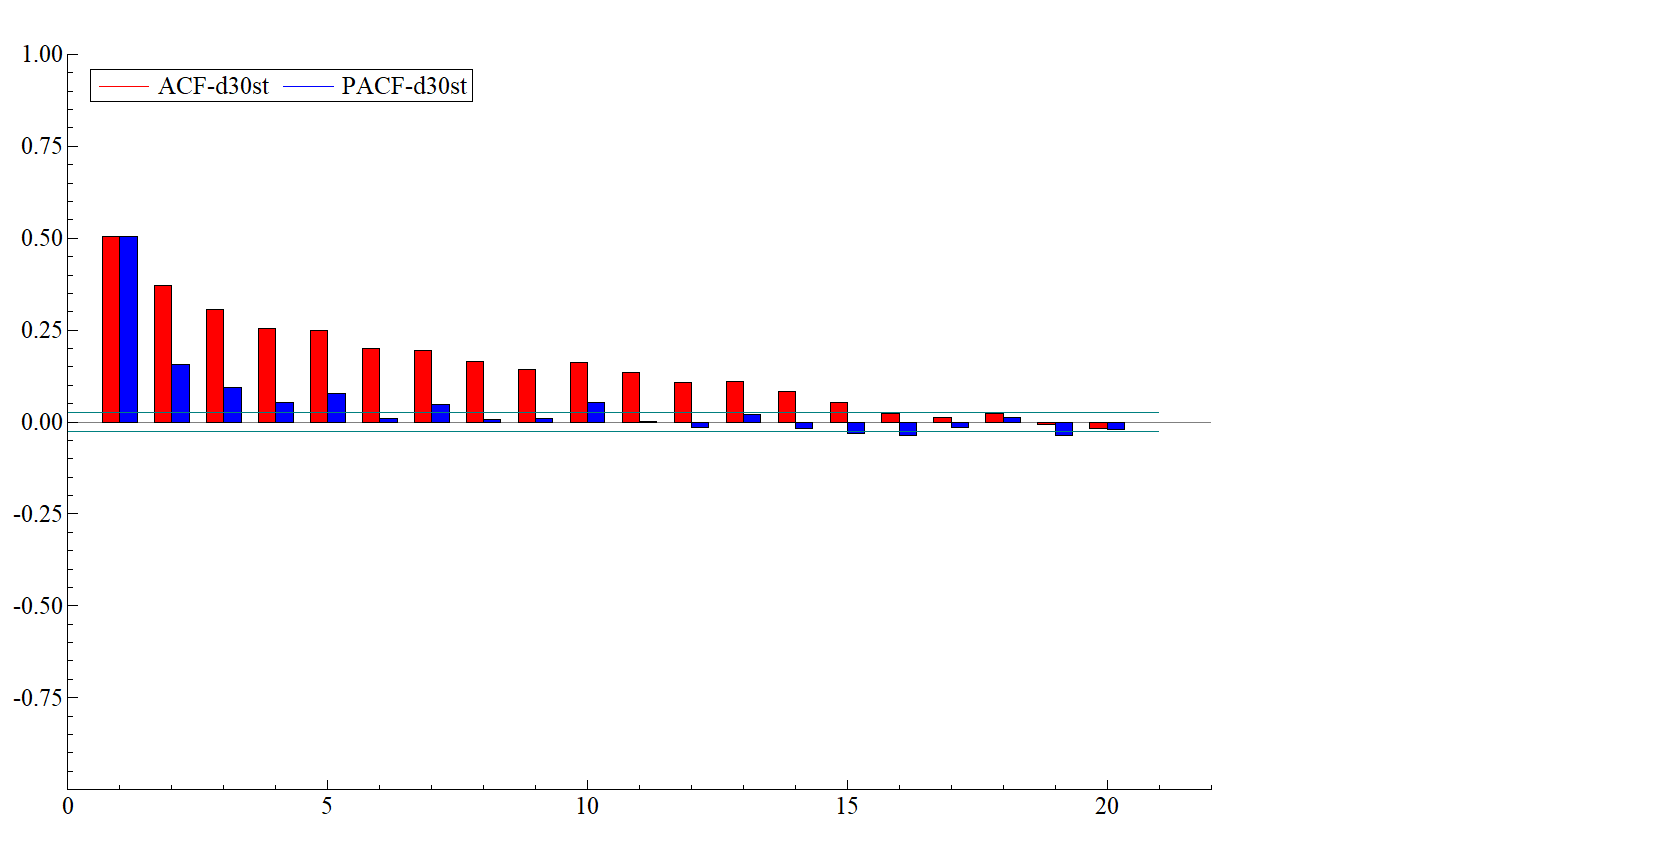
\includegraphics[scale=0.3]{Figure/AFC_model_1.png}
    \caption{Caption}
    \label{fig:my_label}
\end{figure}

\begin{equation}
    S_t = \delta + \sum_{i=1}^{k} \theta_i S_{t-i} + \gramma_1 FirstTrDay_t + \gramma_1 LastTrDay_t + \kappa isJan_t + .... + f_t
\end{equation}

estimating an ar model and saving the resituel as $f_t$

after that I will use the ceil function on the resituels to make the variable into an indicator function. And after that I will multiply it with the ft to get $f^{pos}_t$.

\subsection{part 2 - the GARCH model on stock returns}

here we are going to estimate an GARCH model using the error term from the univariate model above. 

general GARCH model is on the form

\begin{equation}
    y_t = \delta + \theta y_{t-1} + \epsilon_t
\end{equation}

\begin{equation}
    \epsilon_t = \sigma_t Z_t
\end{equation}

conditional variance 

\begin{align}
    \sigma_t^2 = \pi + \alpha \epsilon_{t-1}^2 + \beta \sigma_{t-1}^2  
\end{align}

unconditional variance 

\begin{equation}
    \frac{\pi}{1-\alpha -\beta}
\end{equation}

unconditional mean 

\begin{equation}
    E(y_t) = \frac{\delta}{1-\theta}
\end{equation}

but in this model we have an model that is alternative so the model looks like 

\begin{align}
     y_t = DlogDAX \\
     y_t = \delta + \theta y_{t-1} + \gamma_1 f^{pos}_t + \epsilon_t\\
     \epsilon_t = \sigma_t z_t \\
     \sigma^2_t = \pi + \alpha \epsilon^2_{t-1} + \beta \sigma^2_{t-1}\\
     E(y_t) = \frac{\delta}{1-\theta}\\
     E(y_t, f_t) = \frac{\delta + \gamma_1}{1-\theta}\\
     \sigma^2 = \frac{\pi}{a-\alpha - \beta}\\
\end{align}

we want to investiagate if $\gamma_1 > 0$ so the $H_0: \gramma_1 = 0 $ and the $H_a : \gamma_1 =! 0$.




\newpage






\section{Empirical analysis}




\subsection{The dynamic univariate model}

first we build an auto regressiv model for the st. Start by visuelle evaluation the acf to determind the lag length.



\begin{table}[tbph]
\begin{center}
\begin{tabular}{lrrr}
\hline
& (c) & (w) & (y) \\
\hline
Constant & $\underset{(2.85)}{0.5723}$ & $\underset{(3.13)}{0.314}$ & $\underset{(4.9)}{1.836}$ \\
Trend & $\underset{(2.66)}{0.0003473}$ & $\underset{(2.92)}{0.0004292}$ & $\underset{(4.87)}{0.001084}$ \\
c\_1 & $\underset{(-2.82)}{-0.09223}$ & . & . \\
dc\_1 & $\underset{(-1.77)}{-0.1286}$ & . & . \\
dw\_1 & . & $\underset{(8.44)}{0.5315}$ & . \\
dy\_1 & . & . & $\underset{(-0.88)}{-0.06544}$ \\
w\_1 & . & $\underset{(-3.11)}{-0.05201}$ & . \\
y\_1 & . & . & $\underset{(-4.89)}{-0.2964}$ \\
\hline
$\hat{\sigma}$ & 0.01563 & 0.04424 & 0.02443 \\
Log-lik. & 517.129 & 309.591 & 417.070 \\
\hline
AIC & -5.459 & -3.377 & -4.564 \\
HQ & -5.431 & -3.348 & -4.536 \\
SC/BIC & -5.390 & -3.306 & -4.494 \\
\hline
No autocorr. 1-5 & [0.09] & [0.70] & [0.39] \\
No hetero. & [0.00] & [0.02] & [0.00] \\
Normality & [0.00] & [0.00] & [0.00] \\
\hline
T & 188 & 181 & 181 \\
Sample start & 1971(4) & 1973(3) & 1973(3) \\
Sample end & 2018(3) & 2018(3) & 2018(3) \\
\hline
\end{tabular}
\end{center}
\vspace{1em}
\caption{The table shows estimates of the model in equation (X) with various restrictions imposed. T-ratios in ($\cdot$) and p-values in [$\cdot$] for misspecification tests.}
\end{table}


\newpage

therefor i will use an ar(p) laged model to 

\subsection{Model for daily change in the stock marked}

I will build an GARCH(1,1) model where I include the variable






\section{Conclusion}

}

\end{document}
